\documentclass[12pt,a4paper]{report}

% Packages
\usepackage[utf8]{inputenc}
\usepackage[T1]{fontenc}
\usepackage[lining]{ebgaramond}
\usepackage[cmintegrals,cmbraces]{newtxmath}
\usepackage{microtype}
\usepackage{geometry}
\usepackage{tabularx}
\usepackage{graphicx}
\usepackage{longtable}
\usepackage{booktabs}
\usepackage{array}
\usepackage{listings}
\usepackage{xcolor}
\usepackage{hyperref}
\usepackage{amsmath}
\usepackage{pdflscape}
\usepackage{float}
\usepackage{enumitem}
\graphicspath{{./}}

% Page layout
\geometry{
    left=2.5cm,
    right=2.5cm,
    top=2.5cm,
    bottom=2.5cm
}

% Color definitions
\definecolor{crimson}{RGB}{153, 0, 0}
\definecolor{darkblue}{RGB}{0, 0, 153}

% Hyperlink settings
\hypersetup{
    colorlinks=true,
    linkcolor=crimson,
    urlcolor=crimson,
    citecolor=crimson
}

% Allow line breaks at slashes to prevent overfull hbox
\tolerance=2000
\emergencystretch=2em

% Chapter/section title formatting
\usepackage{titlesec}
\titleformat{\chapter}{\normalfont\huge\bfseries}{}{0pt}{}[\vspace{0.3em}]
\titlespacing*{\chapter}{0pt}{30pt}{20pt}
\titleformat{\section}{\normalfont\Large\bfseries}{\thesection}{1em}{}
\titleformat{\subsection}{\normalfont\large\bfseries}{\thesubsection}{1em}{}

\begin{document}

\pagestyle{plain}

% ─────────────────────────────────────────────
%  Cover Page
% ─────────────────────────────────────────────
\begin{titlepage}
\centering
\vspace*{3cm}

{\fontsize{28}{34}\selectfont\bfseries DSP in VLSI\par}
\vspace{0.6em}
{\fontsize{20}{26}\selectfont\bfseries Homework 1\par}
\vspace{0.4em}
{\fontsize{16}{22}\selectfont\bfseries Sorter\par}

\vspace{1.5cm}
\textcolor{crimson}{\rule{0.6\linewidth}{1.2pt}}
\vspace{1.5cm}

{\large\bfseries Student ID}\par
\vspace{0.4em}
{\large M11407439}\par

\vspace{0.8em}

{\large\bfseries Name}\par
\vspace{0.4em}
{\large MING-HONG, LIN}\par

\vspace{2cm}

{\large\bfseries Development Environment}\par
\vspace{0.8em}
\begin{tabular}{rl}
    \textbf{HDL}      & Verilog HDL \\[4pt]
    \textbf{EDA Tool} & Vivado \\[4pt]
    \textbf{Verification} & Python \\
\end{tabular}

\vfill

\textcolor{crimson}{\rule{0.6\linewidth}{0.6pt}}\par
\vspace{0.5em}
{\small Due Date: 2026/03/18}

\end{titlepage}

% ─────────────────────────────────────────────
%  Table of Contents
% ─────────────────────────────────────────────
\tableofcontents
\newpage

% ─────────────────────────────────────────────
%  Procedure 1
% ─────────────────────────────────────────────
\chapter{Procedure 1 — Testbench Generation}

First, generate several random sequences with 32 elements $[x_1\ x_2\ \ldots\ x_{32}]$
in a block between $-256$ and $255$ as your test inputs and prepare as the testbench. \textbf{(10\%)}

\section{Testbench Input Generation}

For design and verification convenience, instead of generating random sequences
externally via Python or MATLAB, random values in the range of $-256$ to $255$ are
generated directly within the testbench using the expression
\textbf{(\$random \& 9'h1FF) - 256}, and simultaneously written to
\textbf{Input.dat} for subsequent Python-based sorting result verification.

\begin{figure}[h]
    \centering
    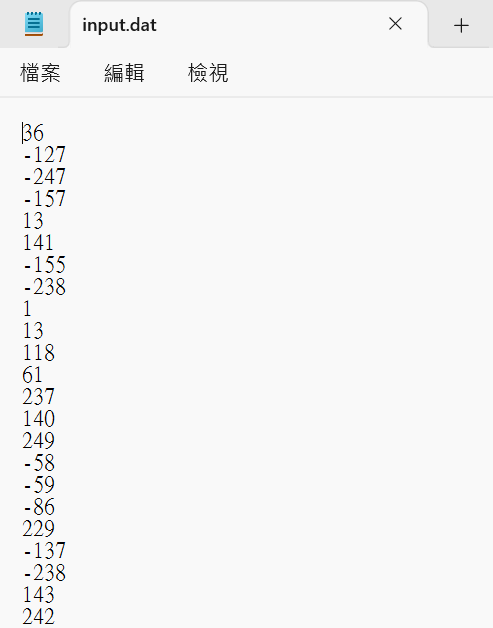
\includegraphics[width=0.5\linewidth]{proc9.png}
    \caption{Content of Input.dat}
    \label{fig:proc9}
\end{figure}


% ─────────────────────────────────────────────
%  Procedure 2
% ─────────────────────────────────────────────
\chapter{Procedure 2 — Sort8 Implementation}

Please use Verilog to implement \textbf{Sort8} with bitonic sorter revised from Fig.~4.
Feed the 8 inputs $[x_1\ x_2\ \ldots\ x_8]$ simultaneously in one clock cycle.
Observe the outputs to realize sorting among eight elements in one group.
Use $[x_1\ x_2\ \ldots\ x_8]$ as the input and check for the correctness of the function
``\textbf{Sort8}'', which can generate sorted output from maximum to minimum.
Indicate this function output in the timing diagram of your behavior simulation results.
(If the data value inside the timing diagram can not be clearly seen, it will not be
regarded as correct answers.) \textbf{(10\%)}

\section{Timing Diagram}
In this Module, due to the excessive combinational comparator path length causing a large critical path delay, two pipeline registers are introduced to reduce the propagation delay per stage, resulting in an output latency of two clock cycles.

\begin{figure}[h]
    \centering
    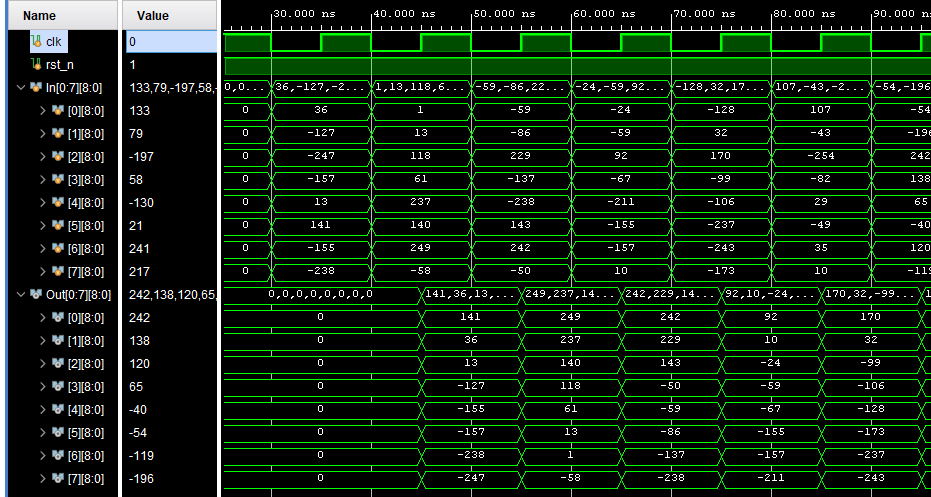
\includegraphics[width=1\linewidth]{proc2.png}
    \caption{Timing Diagram of Sort8 Behavior Simulation Results}
    \label{fig:proc2}
\end{figure}

% ─────────────────────────────────────────────
%  Procedure 3
% ─────────────────────────────────────────────
\chapter{Procedure 3 — SelectTopK Implementation}

Construct the module (\textbf{SelectTopK}) of merger sort to select top~4 among 32 input
elements $([x_1\ x_2\ x_3\ \ldots\ x_{32}])$ under your control.
One example is given as in Fig.~5.
Use a comparator tree to receive the sorted results from each group and then activate
your comparator tree to select top~4 values.
Maybe you need two sets of \textbf{Reg8} buffers, one for saving the outputs of the next
block from Sort8, and the other for sending the contents of the current block to the
comparator tree.

\begin{itemize}
    \item Draw the block diagram of your own implementation and calculate the number of
          adders/subtractors/comparators in your block diagram. \textbf{(20\%)}
    \item Show the timing diagram of your behavior simulation results. \textbf{(10\%)}
    \item Show the hardware output is correct by comparing it to your Matlab (Python)
          results (It means you need to provide the correct answer from the command
          ``sort'' by yourself). \textbf{(10\%)}
\end{itemize}

\newpage

\section{Block Diagram and Calculation}
The Sort8 module uses a total of \textbf{24} comparators, and the bottom-level comparator stage requires an additional \textbf{3}, bringing the overall comparator count to \textbf{27}. As for adders, \textbf{3} are used : one for the Reg Counter that determines which register group to store the Sort8 output into, one for the Pointer adder, and one for the OutRank adder. No subtractors are required.

\begin{table}[H]
    \centering
    \begin{tabular}{ccc}
        \toprule
        \textbf{Comparators} & \textbf{Adders} & \textbf{Subtractors} \\
        \midrule
        27 & 3 & 0 \\
        \bottomrule
    \end{tabular}
    \caption{Component Count of SelectTopK Module}
    \label{tab:proc3-count}
\end{table}

In this module, a Ping-Pong Buffer is employed to maintain high throughput. The first three register groups adopt a full Ping-Pong mechanism, while the last group can be written directly to the Pong Buffer without an additional Ping stage, since its data arrival timing naturally aligns with the output timing and no conflict arises. This allows continuous output of data from different blocks without introducing additional latency.

\begin{figure}[h]
    \centering
    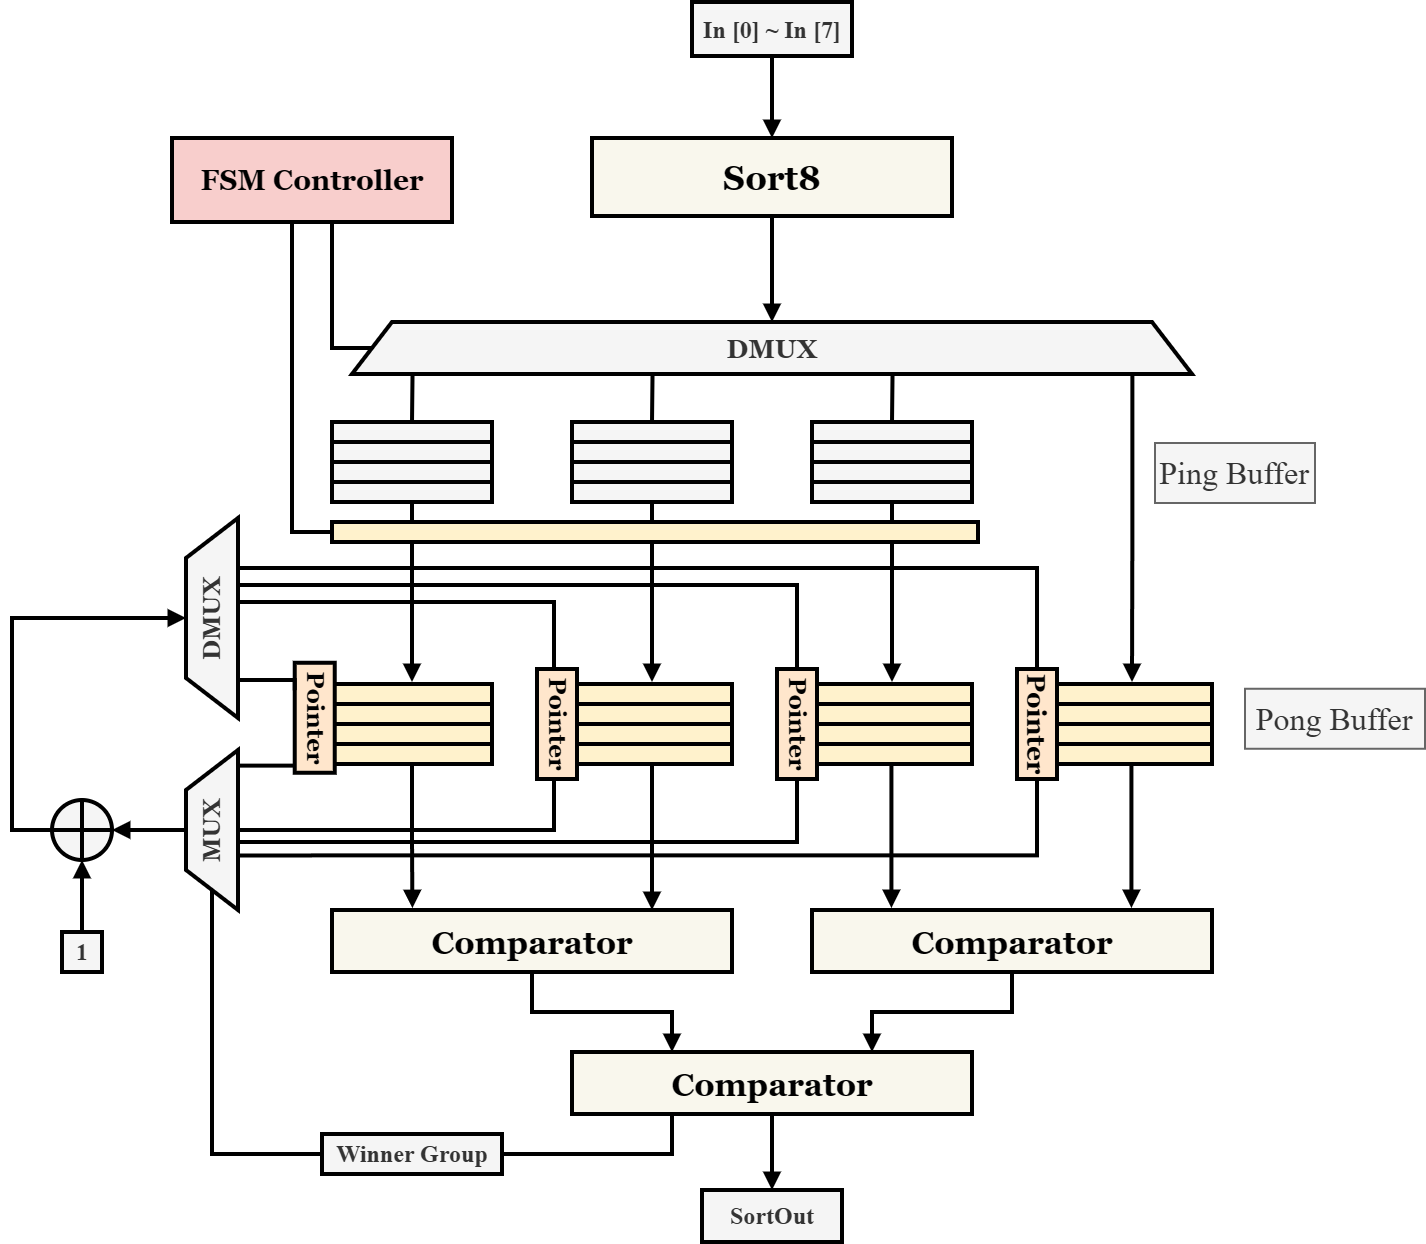
\includegraphics[width=0.85\linewidth]{SelectTopK.png}
    \caption{Block Diagram of SelectTopK}
    \label{fig:proc2}
\end{figure}

\section{Timing Diagram and Verification}

\begin{figure}[h]
    \centering
    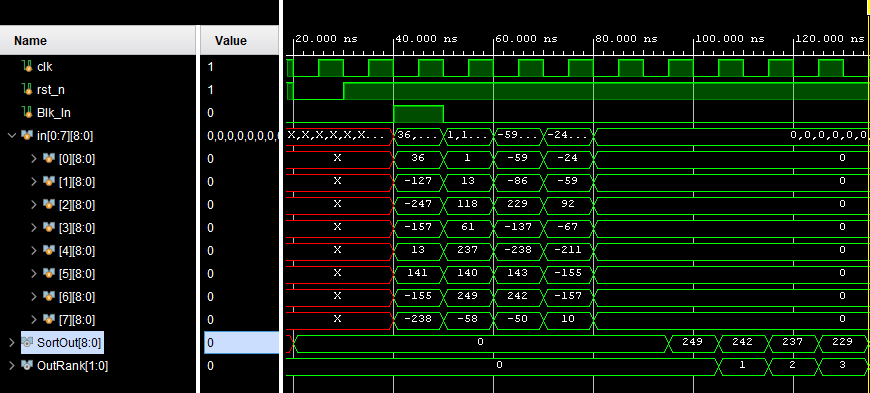
\includegraphics[width=\linewidth]{proc3.png}
    \caption{Timing Diagram of SelectTopK Behavior Simulation Results}
    \label{fig:proc3}
\end{figure}

\begin{figure}[h]
    \centering
    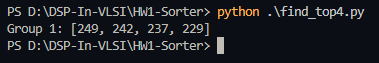
\includegraphics[width=0.5\linewidth]{proc4.png}
    \caption{Sorting Results by Python}
    \label{fig:proc4}
\end{figure}



% ─────────────────────────────────────────────
%  Procedure 4
% ─────────────────────────────────────────────
\chapter{Procedure 4 — Full Timing Verification}

Show that your design can generate required top-4 output in descending order every
4 clock cycles as indicated in Fig.~3 in the timing diagram with proper input signal
``\textbf{BlkIn}'' and output indicator ``\textbf{OutRank}''.
Please feed 4 blocks and check the outputs of four blocks.
If it is too long, please cut it down into several segments to make the numerical
expressions in the timing diagram clear.
If the numerical expressions are hard to distinguish, correct evaluation may not be
given. \textbf{(30\%)}

\section{Timing Diagram}
\begin{figure}[h]
    \centering
    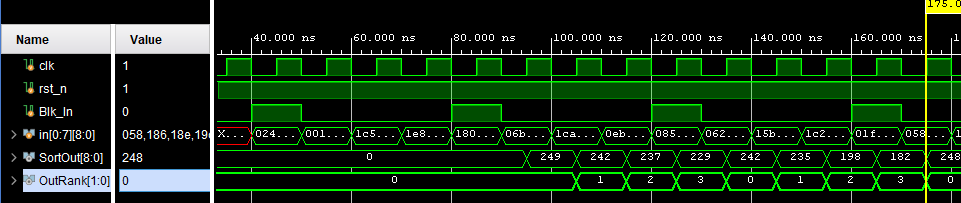
\includegraphics[width=\linewidth]{proc5.png}
    \caption{Timing Diagram of SelectTopK Behavior Simulation Results}
    \label{fig:proc2}
\end{figure}

\begin{figure}[h]
    \centering
    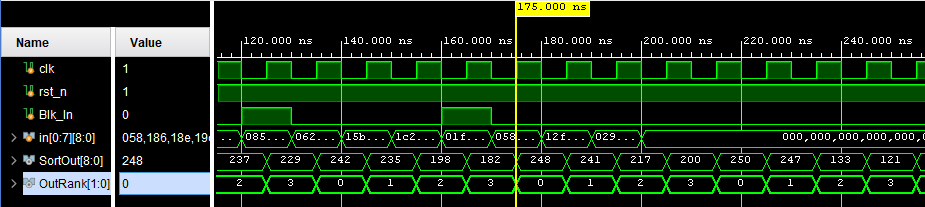
\includegraphics[width=\linewidth]{proc52.png}
    \caption{Timing Diagram of SelectTopK Behavior Simulation Results (Continued)}
    \label{fig:proc2}
\end{figure}

% ─────────────────────────────────────────────
%  Procedure 5
% ─────────────────────────────────────────────
\chapter{Procedure 5 — Python Verification}

Please use Matlab (Python) command ``sort'' to verify your results of your
randomly-generated sequence and compare to the Verilog simulation results. \textbf{(10\%)}

\section{Verification Following Procedure 4}
The sorting results generated by Python \textbf{are identical to} the simulation results from the Verilog simulation in Procedure 4.

\begin{figure}[h]
    \centering
    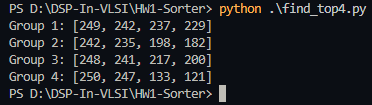
\includegraphics[width=0.5\linewidth]{proc6.png}
    \caption{Sorting Results by Python}
    \label{fig:proc2}
\end{figure}

% ─────────────────────────────────────────────
%  Procedure 6
% ─────────────────────────────────────────────
\chapter{Procedure 6 — Synthesis Report}

Synthesis your design in Procedure~4.
Show the number of adders/subtractors/comparators in your design.
Sum them up together to see if it matches with your block diagram.
\textbf{(10\%)}
(Because you may use counters to control your circuits, we will not ask that the two
values should be exactly the same. However, there should not be a large discrepancy.)

\section{Component Count}
The component counts after synthesis are exactly identical to the estimates from Procedure 3.

\begin{figure}[h]
    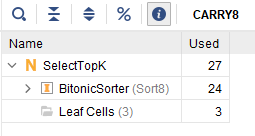
\includegraphics[width=0.3\linewidth]{proc7.png}
    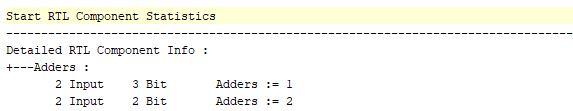
\includegraphics[width=0.7\linewidth]{proc8.png}
    \caption{Component Counts Report}
    \label{fig:proc7}
\end{figure}

\begin{table}[H]
    \centering
    \begin{tabular}{ccc}
        \toprule
        \textbf{Comparators} & \textbf{Adders} & \textbf{Subtractors} \\
        \midrule
        27 & 3 & 0 \\
        \bottomrule
    \end{tabular}
    \caption{Component Count Summary}
    \label{tab:proc3-count}
\end{table}

\end{document}
